\chapter{Detector Installation and Commissioning Organization}
\label{ch:tc-jpo}


As discussed in Chapter~\ref{vl:tc-global}, the \dword{ipd} has
responsibility for coordinating the planning and execution of 
the \dword{lbnf-dune} installation activities both 
in the underground detector caverns at \dword{surf} and 
nearby surface facilities.  The \dword{dune} consortia maintain 
responsibility for their subsystems over the course of these 
activities and provide the expert personnel and specialized 
equipment necessary to integrate, install, and commission their 
detector components.  Likewise, \dword{lbnf} has responsibility 
for activities associated with the installation 
of supporting infrastructure items, which are coordinated under 
the direction of the \dword{ipd}.       

The \dword{jpo} will evolve over time to incorporate the team in South 
Dakota responsible for the overall coordination of onsite
installation activities.  In the meantime, the installation team 
within the \dword{jpo} works with the \dword{dune} consortia 
and \dword{lbnf} project team members to plan these activities.  
%\dword{jpo} installation team members are concurrently embedded within the \dword{dune} \dword{tc} organization during this period to facilitate required interactions with the \dword{dune} consortia. 

The \dword{jpo} installation planning team is 
responsible for specification and procurement of common infrastructure 
items associated with installation of the detectors, 
which are not included within the scope of the \dword{dune} consortia.  
Some of these items are detector pieces such as racks, cable trays, cryostat 
flanges and mechanical structures for supporting the detectors within 
the cryostats.  Others are general items required for detector
installation such as clean rooms, cranes, scaffolding and personnel 
lifts.
%Within its support role, \dword{dune} \dword{tc} works closely with the \dword{jpo} team to characterize these items and contributes engineering resources for required design efforts.

The onsite \dword{jpo} team includes rigging 
teams responsible for moving materials in and out of the shaft, through the 
underground drifts, and within the detector caverns.  It includes
personnel responsible for overseeing safety and logistics planning.  These 
team members are anticpated to sit within the \dword{sdsd}, an organization 
formed to provide \dword{fnal} support services in South Dakota.    

\section{Far Site Safety}
\label{sec:far_site_safety}

The foundation of a credible installation plan is an \dword{esh}
program that ensures the safety of team members and
equipment supporting the program, and protection of the environment at
the \dword{surf} site.  The \dword{ipd} has responsibility for
implementing the \dword{lbnf-dune} \dword{esh} program for 
installation activities in South Dakota.  The \dword{lbnf-dune}
\dword{esh} manager heads the onsite safety organization and reports
to the \dword{ipd} to support the execution of this
responsibility.

The far site \dword{esh} coordinators sitting under the
\dword{lbnf-dune} \dword{esh} manager oversee the day-to-day execution
of the installation work as shown in
Figure~\ref{fig:dune_esh_installation} and is described further in
Chapter~\ref{vl:tc-ESH}.
\begin{dunefigure}[\dword{dune} installation \dword{esh}]{fig:dune_esh_installation}
  {High level \dword{dune} installation \dword{esh} organization.}
  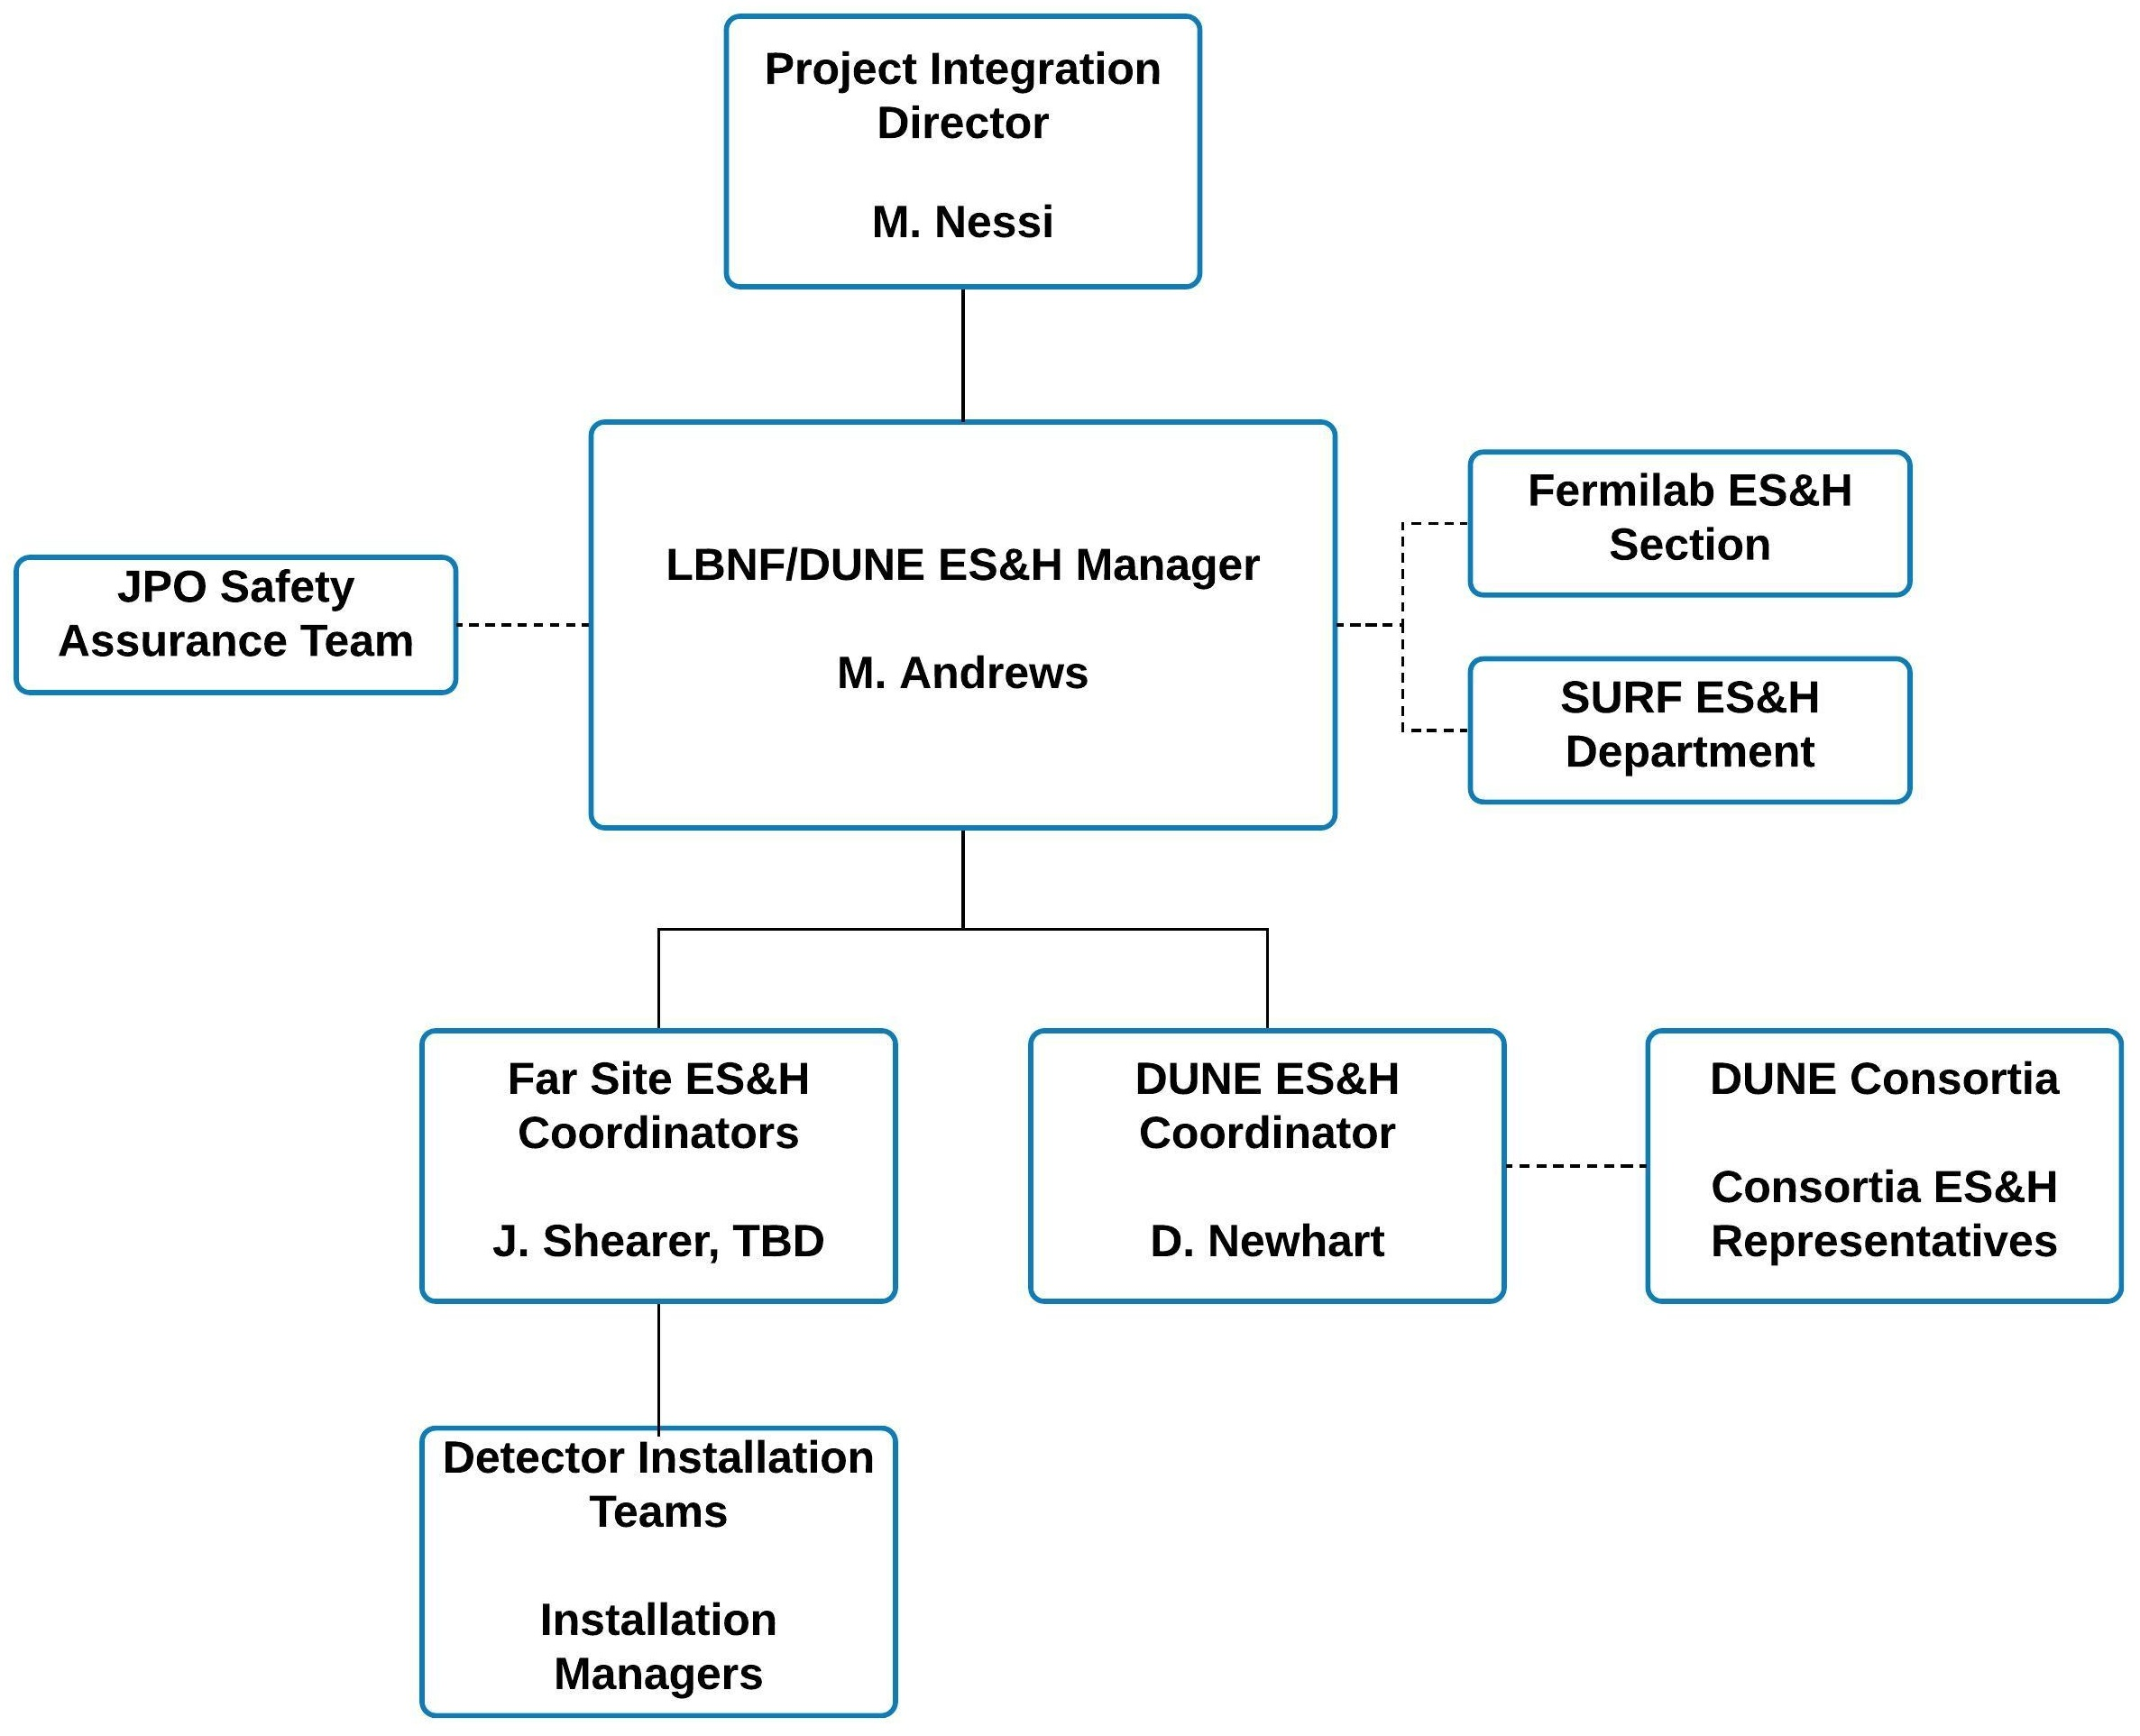
\includegraphics[width=0.85\textwidth]{DUNE_Installation_Safety_OrgChart}
\end{dunefigure}
As we move to 2-shift installation activity,
additional far site \dword{esh} coordinators will be assigned to each
work shift.  The safety coordinator assigned
to a particular shift is responsible for leading safety
discussions during the toolbox meeting and for
ensuring that all workers on that shift, including those from the
consortia or contractors, are properly trained.  The reporting chain for safety
incidents goes through the onsite safety team to the
\dword{lbnf-dune} \dword{esh} manager to minimize any potential
conflicts of interest.  All \dword{jpo} installation team members as
well as \dword{dune} consortia personnel and \dword{lbnf} project team
members have the right to stop work for any safety issues.

Operation of all equipment used for installation activities such as
cranes, power tools, and personnel lifts is restricted to team members
who have been properly trained and certified for use of that
equipment.  The safety coordinator for each shift is responsible for
ensuring that all team personnel are properly trained and that safety
documentation and work procedures are up-to-date and stored within the
\dword{edms}.

Documentation, including accident reports, near misses, weekly
reports, equipment inspection, and training records is an important
component of the \dword{lbnf-dune} \dword{esh} program. The work
planning and \dword{ha} program utilizes detailed work plan documents,
\dword{ha} reports, equipment documentation, safety data sheets,
\dword{ppe} and job task training to mimimize work place hazards and
maximize efficiency.  Sample documentation is developed through the
\dword{ashriver} trial assembly process, which maps out the step by
step procedures and brings together the documenation needed for
approving the work plan.  The sample documentation is modified to
account for differences required for performing work underground and
the updated procedures are provided to the review process (as
discussed in Chapter~\ref{vl:tc-review}) for \dwords{irr} and
\dwords{orr}.

\section{JPO Management}
\label{vl:tc-facility_mgmt}

The \dword{ipd} is responsible for coordinating all installation
activities at \dword{surf} including those that fall under the direct
responsibility of \dword{lbnf} and the \dword{dune} consortia.  The
coordinators of this activity and crucial technical support
staff sit within the \dword{jpo}.  The organization of this onsite
team is shown in Figure~\ref{fig:ash_river}.
\begin{dunefigure}[far site organization chart]{fig:ash_river}
  {far site organization chart}
  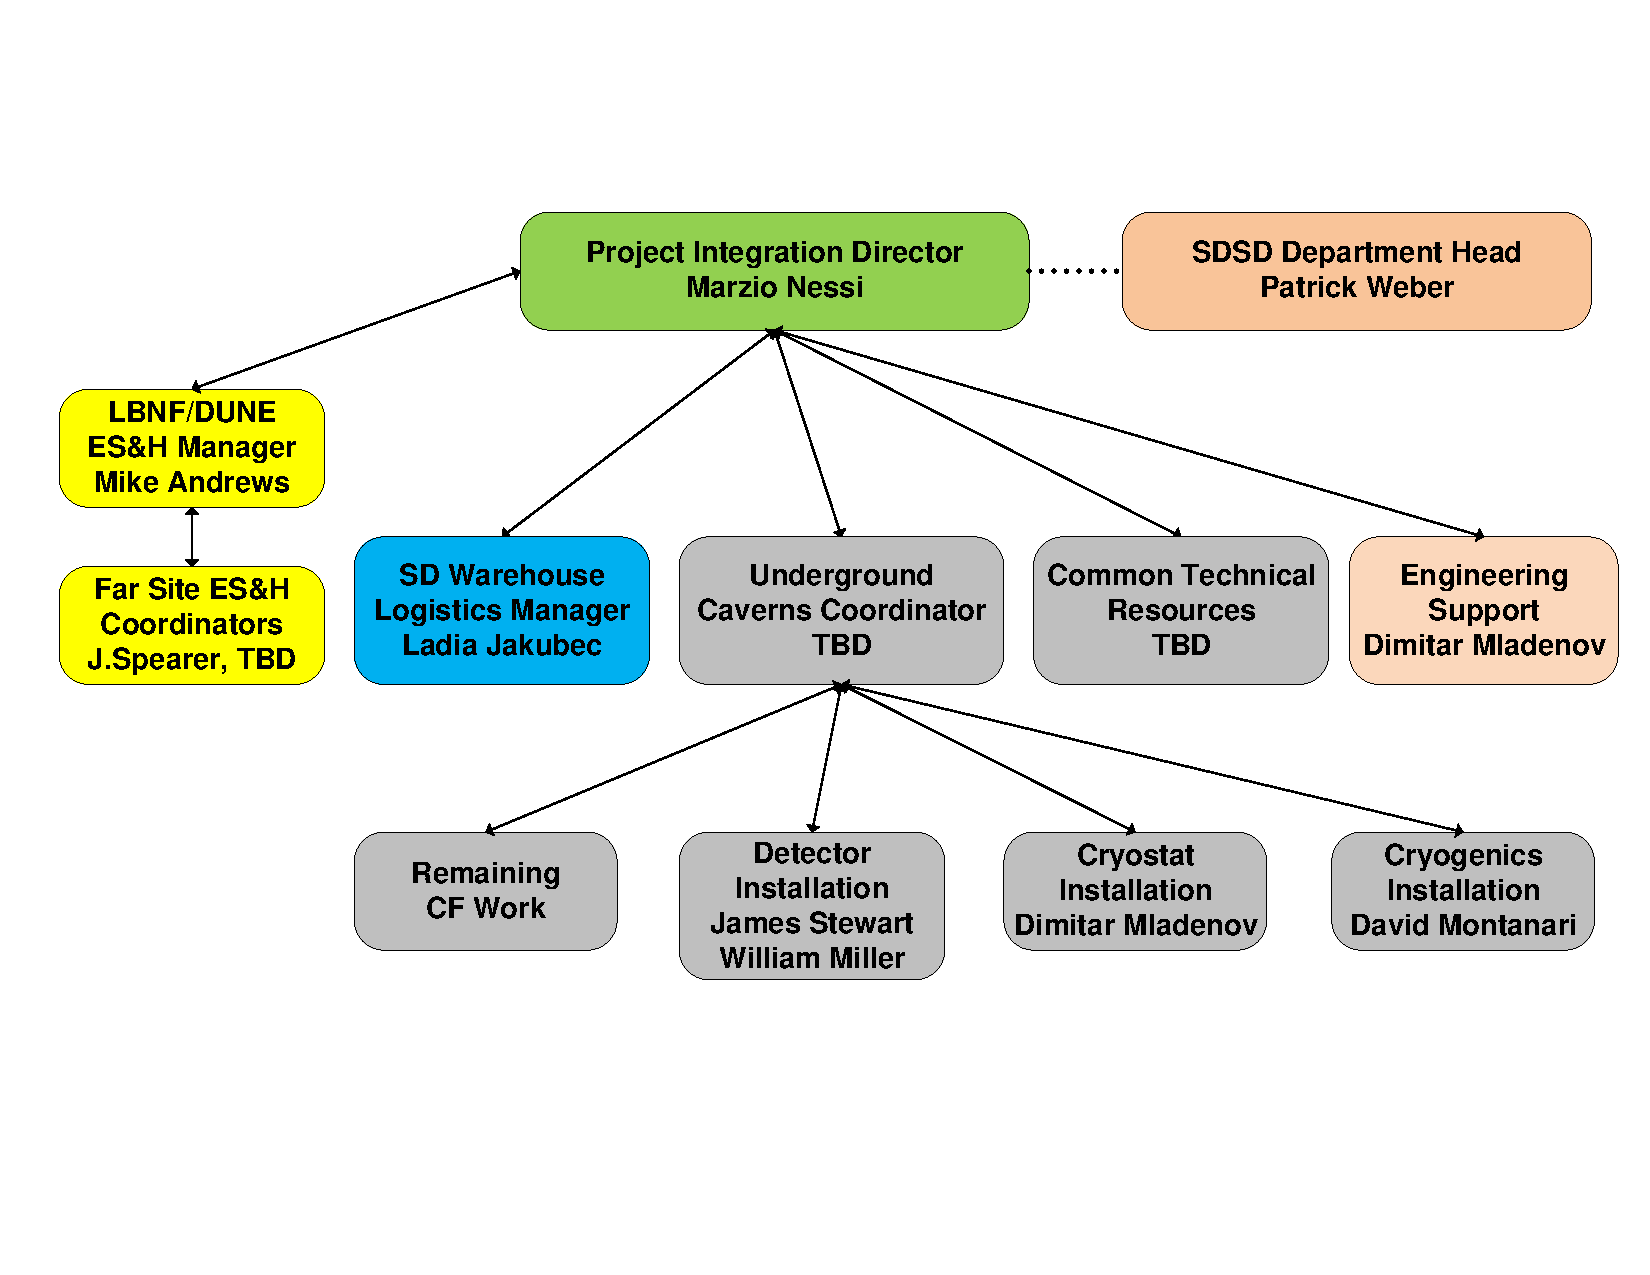
\includegraphics[width=0.95\textwidth]{Org-Far-Site-TDR-10-9-19}
\end{dunefigure}
 
As discussed in Section~\ref{sec:far_site_safety} the onsite safety
organization including the far site \dword{esh} coordinators
working under the direction of the \dword{lbnf-dune} \dword{esh}
manager oversee all onsite activites and have a direct reporting line
to the \dword{ipd}.

Due to the lack of surface space at \dword{surf}, a separate
warehousing facility in the vicinity of \dword{surf} is required to
receive and store materials in advance of their delivery to the
undergound area as discussed in Section~\ref{sec:sdwf}.  Warehouse
operations are coordinated by the \dword{lbnf-dune} logistics manager
who is tasked with determining the exact sequence in which materials
are delivered into the underground areas.

The underground cavern coordinator is responsible for managing all 
activities in the two undergound detector caverns as well as the
\dword{cuc}, this includes contracted workers.  Work within the
detector caverns follows a time ordered sequence that includes
installation of the cryostats (warm and cold), cryogenic systems, and
the detectors themselves.  Work in the \dword{cuc} includes
installation of major cryogenic system pieces and the detector
\dword{daq} electronics.  The underground cavern coordinator relies on
separate installation teams focusing on cryostats, cryogenic systems,
and the detectors.  The cryostat and cryogenics system installation
teams are contracted resources provided by \dword{lbnf}.  For this
reason, coordinators of these activities are embedded within both the
\dword{lbnf} project team and the \dword{jpo}.  The detector
installation teams incoporate a substantial number of scientific and
technical personnel from the \dword{dune} consortia.  Coordinators of
the detector installation effort sit within the \dword{jpo}
during the period when these activities are being executed.  Any
modifications to the facilities occuring after \dword{aup} are managed
by the underground cavern coordinator under the direction of the
\dword{ipd}.

The \dword{ipd} manages common technical and engineering resources to
support installation activities.  Technical resources include the
support crews needed for rigging materials on and off the hoist at the
top and bottom of the shaft, transporting materials to the underground
caverns from the bottom of the shaft, and rigging the detector and
infrastructure pieces within the underground caverns during the
installation process.  Additional, common technical resources used
across the installation efforts are welders and survey teams. Access
to on-call electricians and plumbers is required to support the
installation effort and deal with operational issues as they arise.
Required technical resources described here are provided through 
\dword{sdsd}, which will employ full-time staff members and contracted
support staff to provide the necessary functions.

Engineering resources for installation activities sit within
the \dword{jpo}.  The engineering team, which includes both mechanical
and electrical engineers, resolves last minute issues associated with
component handling and detector grounding that arise over the course
of the installation process.  Other required engineering functions
include procurement support, configuration management, and
particpation in the safety review process.

\subsection{South Dakota Warehouse Facility}
\label{sec:sdwf}

The \dword{sdwf} is a leased 5000m$^2$ facility hosted by 
\dword{sdsd}.  Approximately six months before \dword{aup}
of the underground detector caverns is received, the \dword{sdwf} 
is required to be in place for receiving cryostat and detector 
components.  Laydown space near the Ross headframe is extremely 
limited.  For this reason, the transportation of materials from 
the \dword{sdwf} to the top of the Ross shaft requires careful 
coordination. The \dword{lbnf-dune} logistics manager works with 
the \dword{cmgc}, through the end of excavation activities, and 
the other members of the \dword{jpo} team to coordinate transport 
of materials into the underground areas.  Since no materials or 
equipment can be shipped directly to the Ross or Yates headframes, 
the \dword{sdwf} is used for both short and long-term storage, as 
well as for any re-packaging of items required prior to transport 
into the underground areas. 

A small number of \dword{dune} consortia members work at the
\dword{sdwf} to check received components for potential damage
incurred during shipment and track all materials coming in and out of
the facility, using the inventory management system.  In some cases
re-packaging of materials is required for lowering them down the shaft
into the underground areas.  The \dword{dune} consortia take
responsibility for these efforts.

\subsection{Underground Caverns}

The installation 
process in the underground detector caverns and \dword{cuc} can 
be broken into a time-sequenced set of activities, coordinated 
through the \dword{jpo}.  In the detector caverns, installation 
of the warm and cold cryostat strucutres is followed by (with 
some overlap) installation of the cryogenic infrastructure and 
detectors.  In the \dword{cuc} installation of the \dword{daq}  
infrastructure and detector readout components proceeds in 
parallel with that of the cryogenic infrastructure.  A high-level 
schedule showing the inter-dependencies between these activities 
is shown in Figure~\ref{fig:underground_schedule}.
\begin{dunefigure}[Underground summary schedule]{fig:underground_schedule}
  {Summary schedule of the different phases of work underground}
  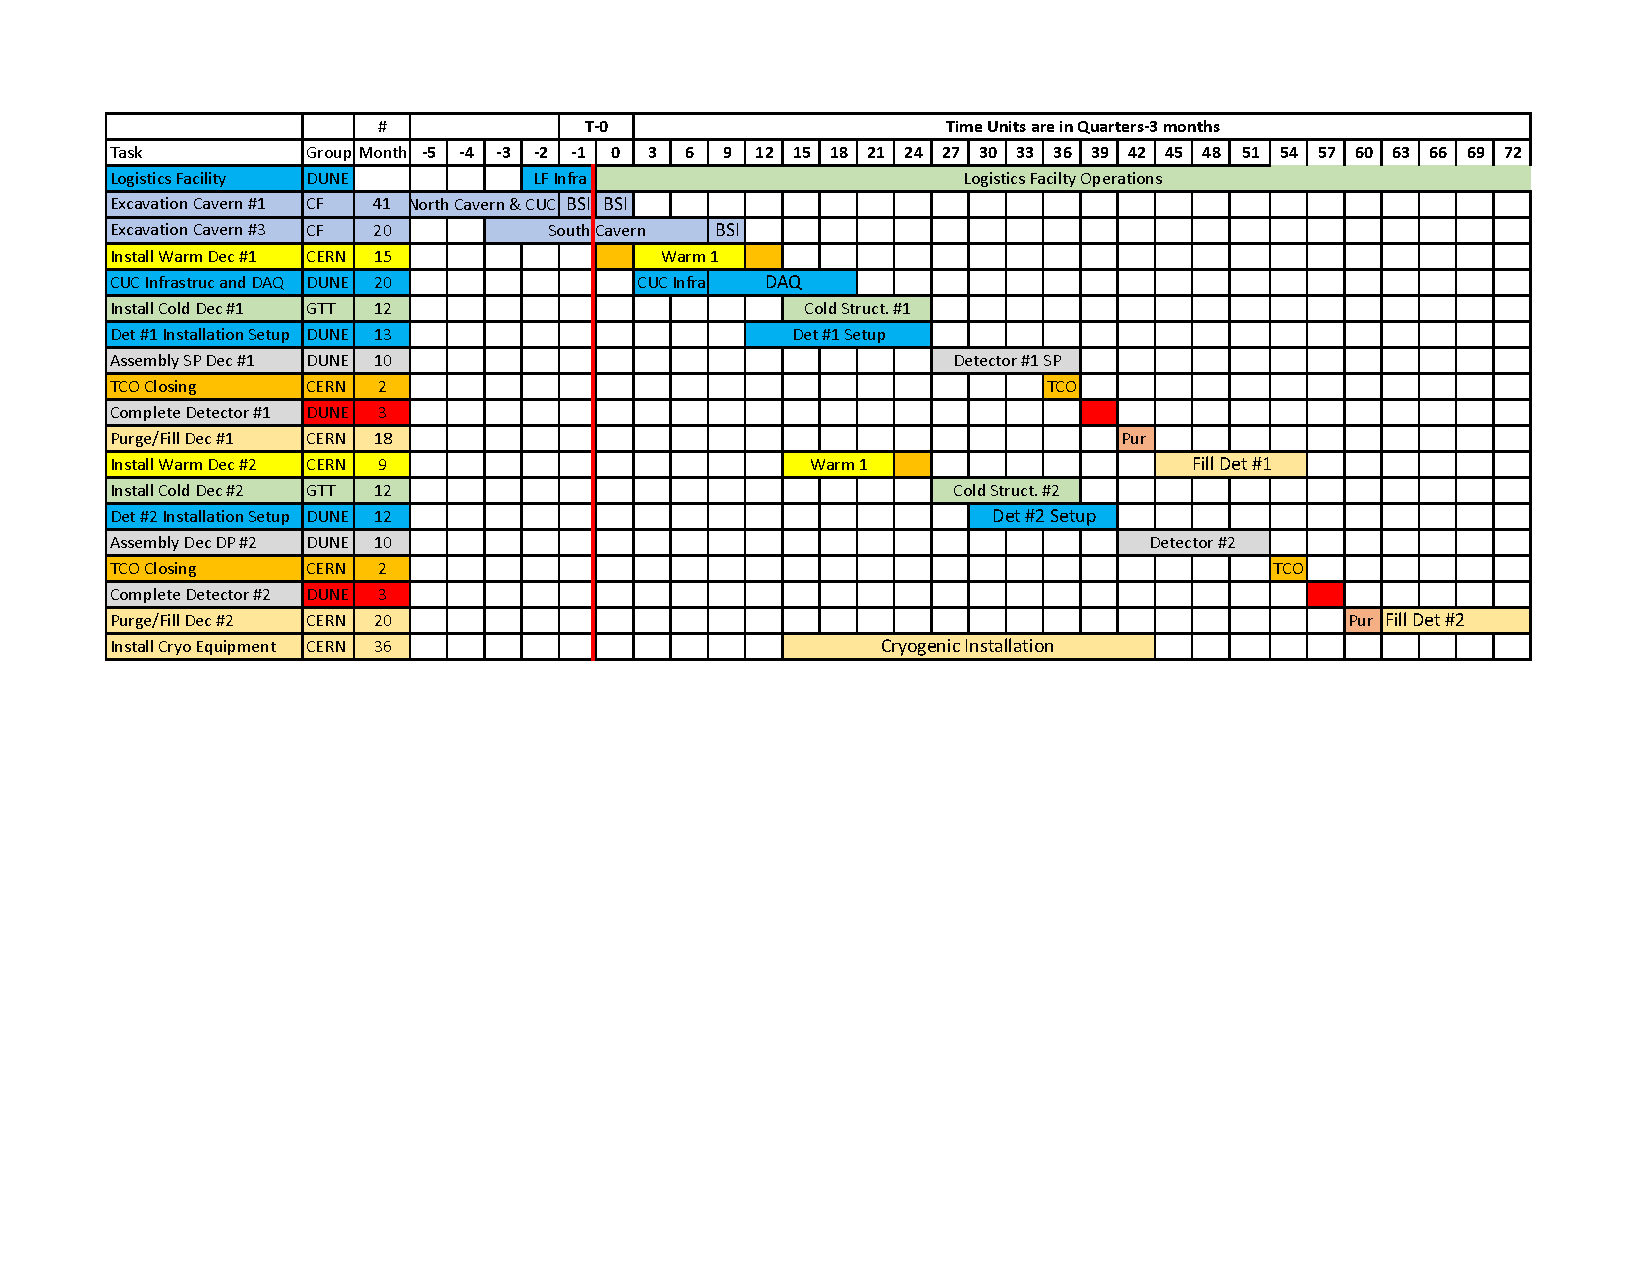
\includegraphics[width=0.95\textwidth]{Overall_schedule-T0}
\end{dunefigure}

The ability of \dword{lbnf-dune} to meet this schedule depends
critically on its ability to work within limitations on the total
number of people allowed in the underground areas at a given time
(144) as well as occupancy limits on work in the cryostat.  In order
to satisfy these limitations, careful balancing of the numbers of
workers assigned to different concurrent tasks taking place within the
different underground caverns is required.  This is a particular
challenge during the excavation period for the second detector cavern,
which runs in parallel with cryostat installation in the first
detector cavern.  The \dword{jpo} works with its
\dword{lbnf-dune} project partners to manage and optimize the
underground work schedule so that interferences between concurrent
work efforts are minimized.

The underground cavern coordinator manages the contributions of 
the technical team supporting the installation activities.
The size of the technical support team is anticipated to evolve  
over time to meet the needs of the specific installation tasks 
taking place.  The functions provided by the technical team 
supporting the work in the underground caverns include the
following:
\begin{itemize}
  \item {material transport:} The transport team shown in
    Figure~\ref{fig:ctr_orgchart} is responsible for unloading of
    materials from the trucks arriving from the \dword{sdwf}, loading
    or rigging of materials at top of Ross Shaft, unloading or rigging
    of materials at bottom of Ross Shaft, and delivery of materials
    from the bottom of shaft to the underground caverns. This does not
    include operation of the hoists which is performed by
    \dword{surf}.
  \item {cavern rigging operations:}  Storage of 
        components within the available spaces 
        in the cavern and movement of materials as required to 
        execute the installation process (three rigging stages
        for detector installation are moving components into 
        clean room, integrating components within clean room, 
        and installing integrated elements inside cryostat).
  \item {installation technicians:}  General technician 
        support for specific installation activities. 
  \item {welders and survey crews:}  Perform 
        specific tasks incorporated within each of the different 
        installation efforts.
  \item {electrical technicians and plumbers:} On-call support staff
    to modify systems as work transitions from one stage to the next
    and to address issues as they arise.
\end{itemize}   
    
The organization responsible for managing contributions of 
the technical support team to the installation 
activities taking place in the underground caverns is shown 
in Figure~\ref{fig:ctr_orgchart}.  The structure is illustrated
for the case of the largest anticipated workforce (approaching 
roughly sixty team members in total covering multiple shifts) 
for the periods with ongoing detector installation efforts.
These personnel support two 10-hour shifts on Mondays through 
Thursdays and a day shift on the remaining days to cover 
activities occuring over weekends. 
\begin{dunefigure}[Common Technical Resources]{fig:ctr_orgchart}
  {Summary of the \dword{jpo}/\dword{sdsd} Common Technical Resources}
  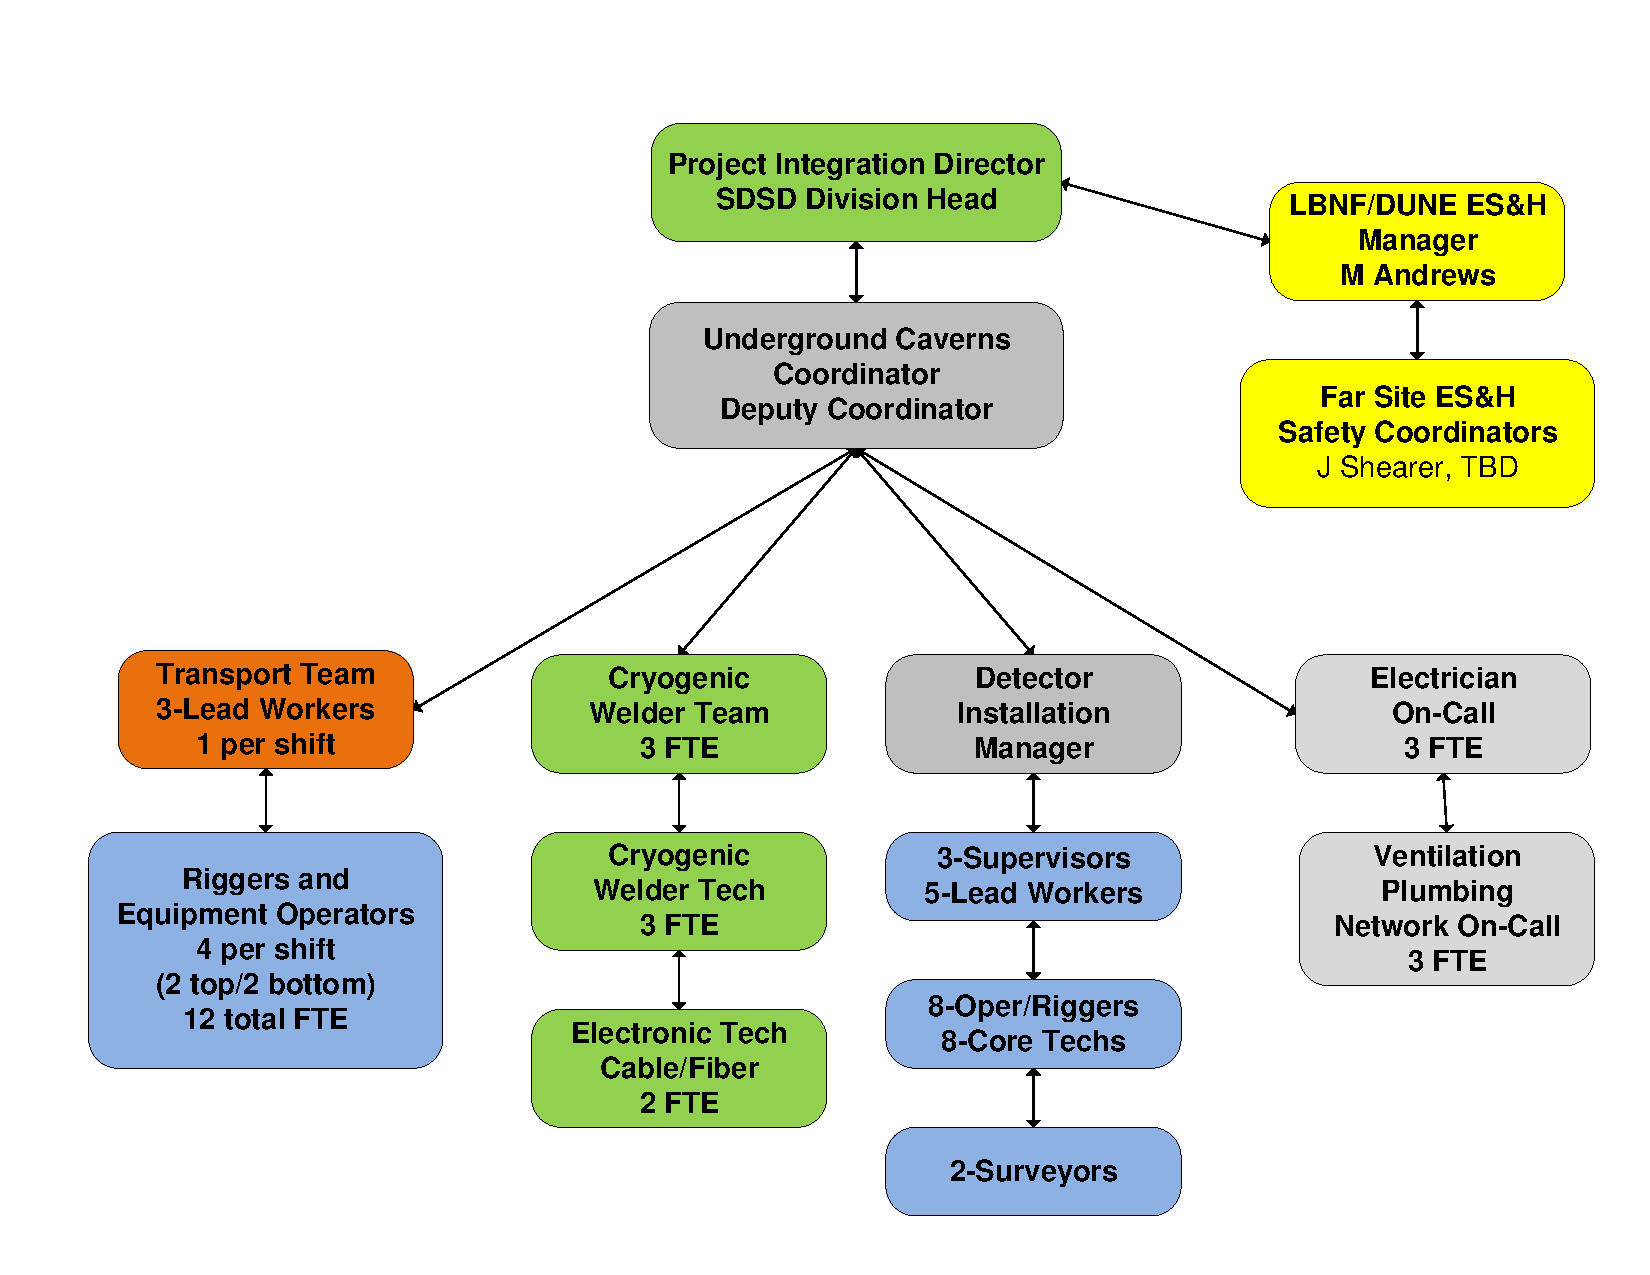
\includegraphics[width=0.95\textwidth]{Org_Technical_Resources-JPO-TDR-10-9-19}
\end{dunefigure}

On the surface at the start of each shift, there is a toolbox safety
meeting and work assignment update. An hour separates the two shifts,
in which the lead workers, safety coordinators, and other management
team members, are paid overtime to overlap with each other and
transfer information from one shift to the next. The safety
coordinator for each shift is responsible for conducting the safety
discussion at the meeting and ensuring that all workers assigned to
that shift have the proper trainings.

The team responsible for detector installation incorporates 
members of the technical support team described above 
and includes scientific and technical personnel from 
the \dword{dune} consortia.  The team is led by the detector
installation manager who has three shift supervisors working 
with him or her to provide onsite coverage for every shift.
The management team works with the underground cavern
coordinator to ensure that required technical support team 
members are available as needed and that required materials 
are delivered to the detector caverns on a schedule to keep
the installation effort moving forward.         

The management team supervises technical resources assigned to 
the detector installation effort and works with consortia 
team members to maximize the overall efficiency of the installation 
process.  The organizational structure to manage the detector 
installation activities is shown in Figure~\ref{fig:uit_orgchart}.
\begin{dunefigure}[Underground detector installation team]{fig:uit_orgchart}
  {The \dword{uit}}
  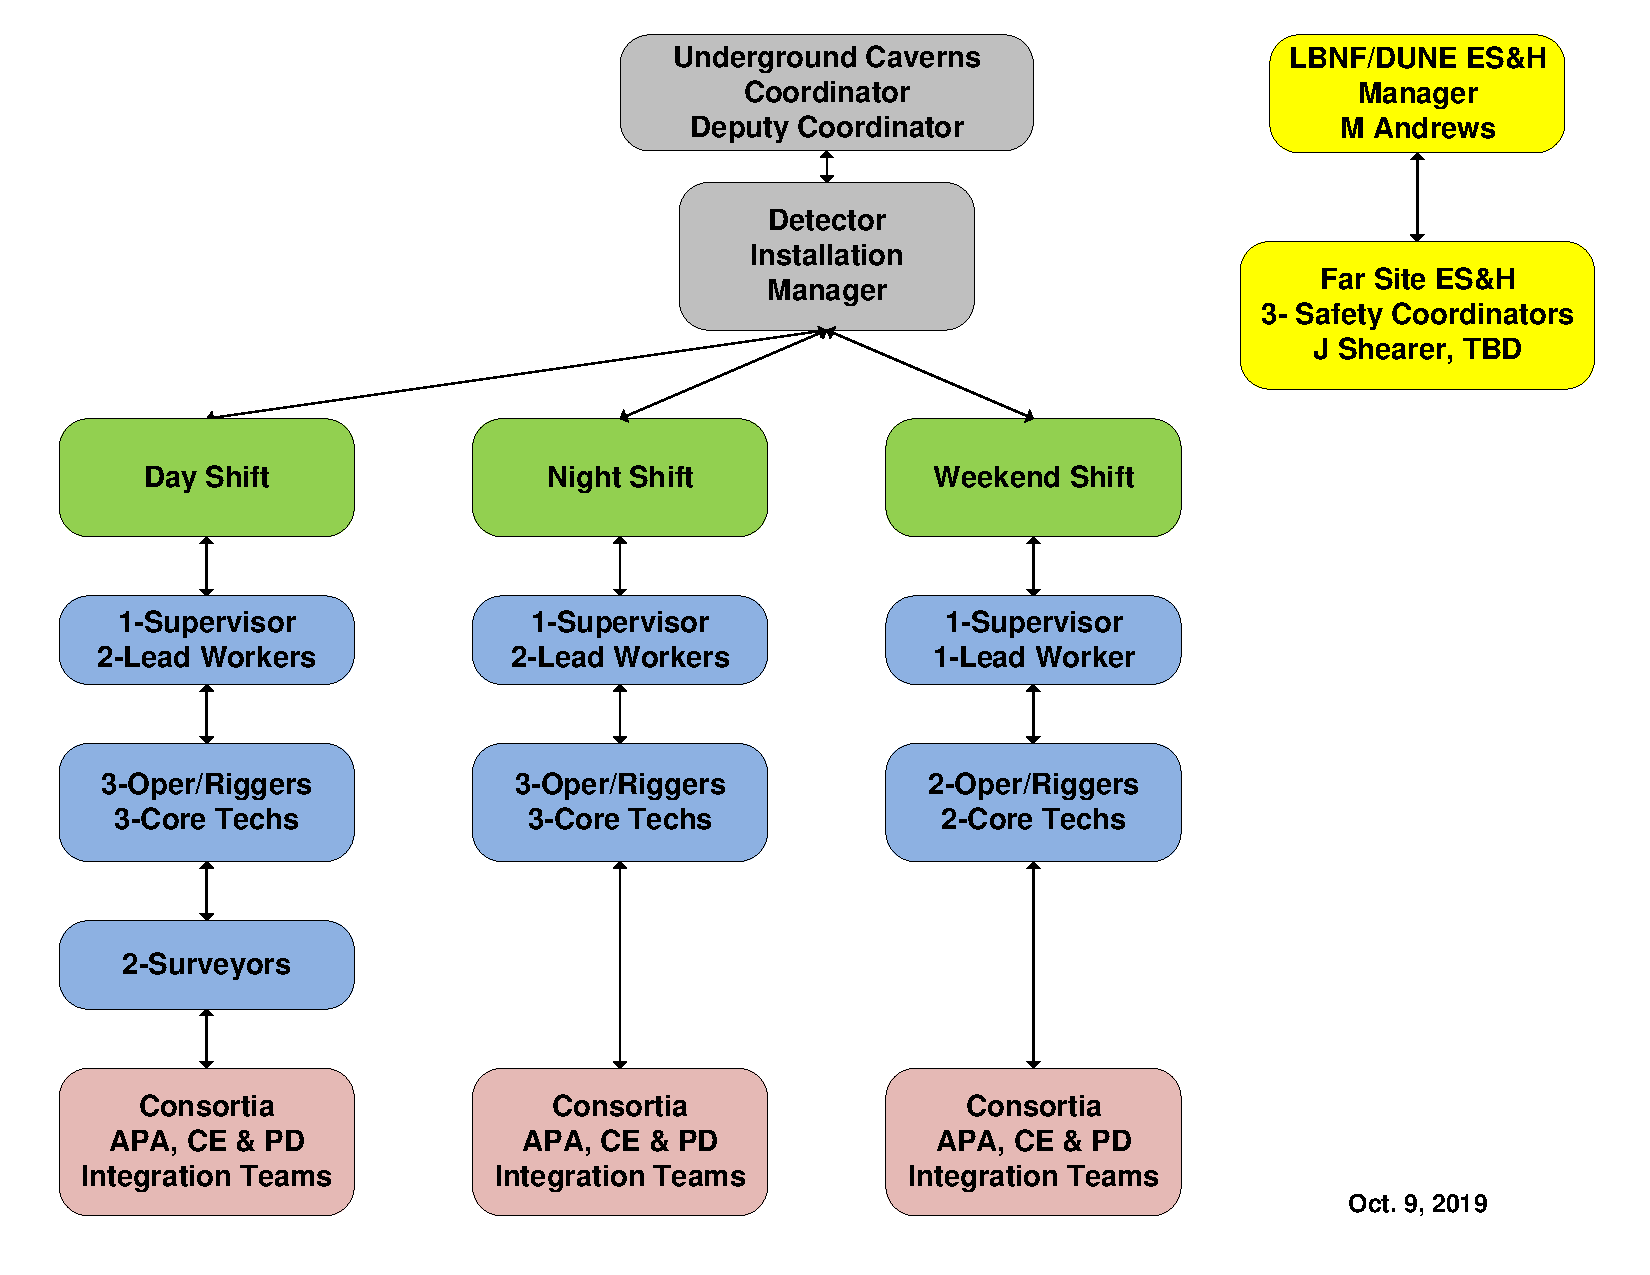
\includegraphics[width=0.95\textwidth]{Org_UIT-TDR-10-9-19}
\end{dunefigure}

The detector installation manager oversees all shifts and serves as
the supervisor for specific shifts as needed.  They serve as the
contact with the underground cavern coordinator for obtaining
required technical support team members and organizing the delivery of
needed materials into the detector caverns.  The detector installation
manager attends all high-level meetings with the underground cavern
coordinator and is tasked with submitting weekly progress reports.
They work with the \dword{dune} consortia to manage the overall work
schedule and ensure that the correct resources are in the right place
at the right time.
    
The installation supervisors are working managers, trained as riggers
and equipment operators to fill in as needed on their shifts.  They
are fully trained in all installation procedures and work with the
consortia shift team members to keep the installation effort on
schedule.  Installation supervisors fill in for their lead workers as
needed and are the primary points of contact for information exchange
between shifts.  Lead workers direct the technical support personnel
assigned for their shift.  The lead workers are trained in all
installation procedures and provide assistance to the consortia work
teams as needed.

\subsection{Trial Assembly at \dword{ashriver}}

The trial assembly work at \dword{ashriver}, site of the \dword{nova}
far detector, focuses on mechanical tests of the installation
process for \dword{dune}. This effort is critical to confirm final
detector component designs, including modifications originating from
\dword{protodune}. It confirms and practices installation techniques
for both the cleanroom and cryostat.  The \dword{nova} far site
detector hall in Ash River, Minnesota has facilities that
match \dword{dune} needs, including a \SI{16.75}{m} deep pit with
$\sim$\SI{300}{m$^2$} of floor space available for testing full-scale
\dword{dune} detector components and a capable workforce that is
needed for \dword{nova} operations and can be leveraged in a cost effective
manner for \dword{dune}.  The \dword{nova} far detector Laboratory is
managed by the University of Minnesota (UMN) and is partially funded
through an operations contract from \dword{fnal}.  Work performed at
the \dword{ashriver} site follows university safety regulations and
any \dword{dune} safety requirements University code officials approve
all building permits, which include engineered drawings signed by an
engineer registered in Minnesota. All hazard analyses and work
procedure documents are approved by the joint \dword{dune}/UMN safety
committee with members drawn from both the University of Minnesota
(UMN) and \dword{dune} that includes specialists as needed.

The work at \dword{ashriver} has five main goals:
\begin{itemize}
  \item using prototype \dword{dune} components, verify that the
    \dword{dune} detector can be installed in a safe and efficient
    manner,
    \item test installation equipment needed to install the
      \dword{dune} detector at \dword{surf},
  \item validate mechanical design changes made to the detector
    elements subsequent to \dword{protodune} operation,
  \item complete a set of reviewed engineering and procedural
    documents that will serve as the basis for work to be performed
    underground at \dword{surf}, and
  \item serve as a training center for personnel who will 
    contribute to \dword{dune}  installation at \dword{surf}.
\end{itemize}

The full time staff of five people at \dword{ashriver}
includes a manager, deputy manager, and three experienced technicians
that all participated in \dword{pdsp} installation at \dword{cern} and
the \dword{pdsp} trial assembly at \dword{ashriver}.  The staff
oversees operations of the \dword{nova} detector and performs trial
assembly studies of the \dword{dune} detector components.  One of the
three technicians also serves as the site safety officer and
chairperson of the joint \dword{dune}/UMN safety committee.  Two additional staff
members will be added in the near future to handle the additional
workload associated with preparations for the \dword{protodune2}
installation effort.
\begin{dunefigure}
  [Phase 1 \dword{apa} installation frame being installed on
    the \dword{apa} assembly tower at \dword{ashriver}]{fig:ashriver1}
  {Phase 1 \dword{apa} installation frame (in red) being installed on the
  \dword{apa} assembly tower at \dword{ashriver}. In the foreground is
  the \dword{pdsp} trial assembly structure.}
   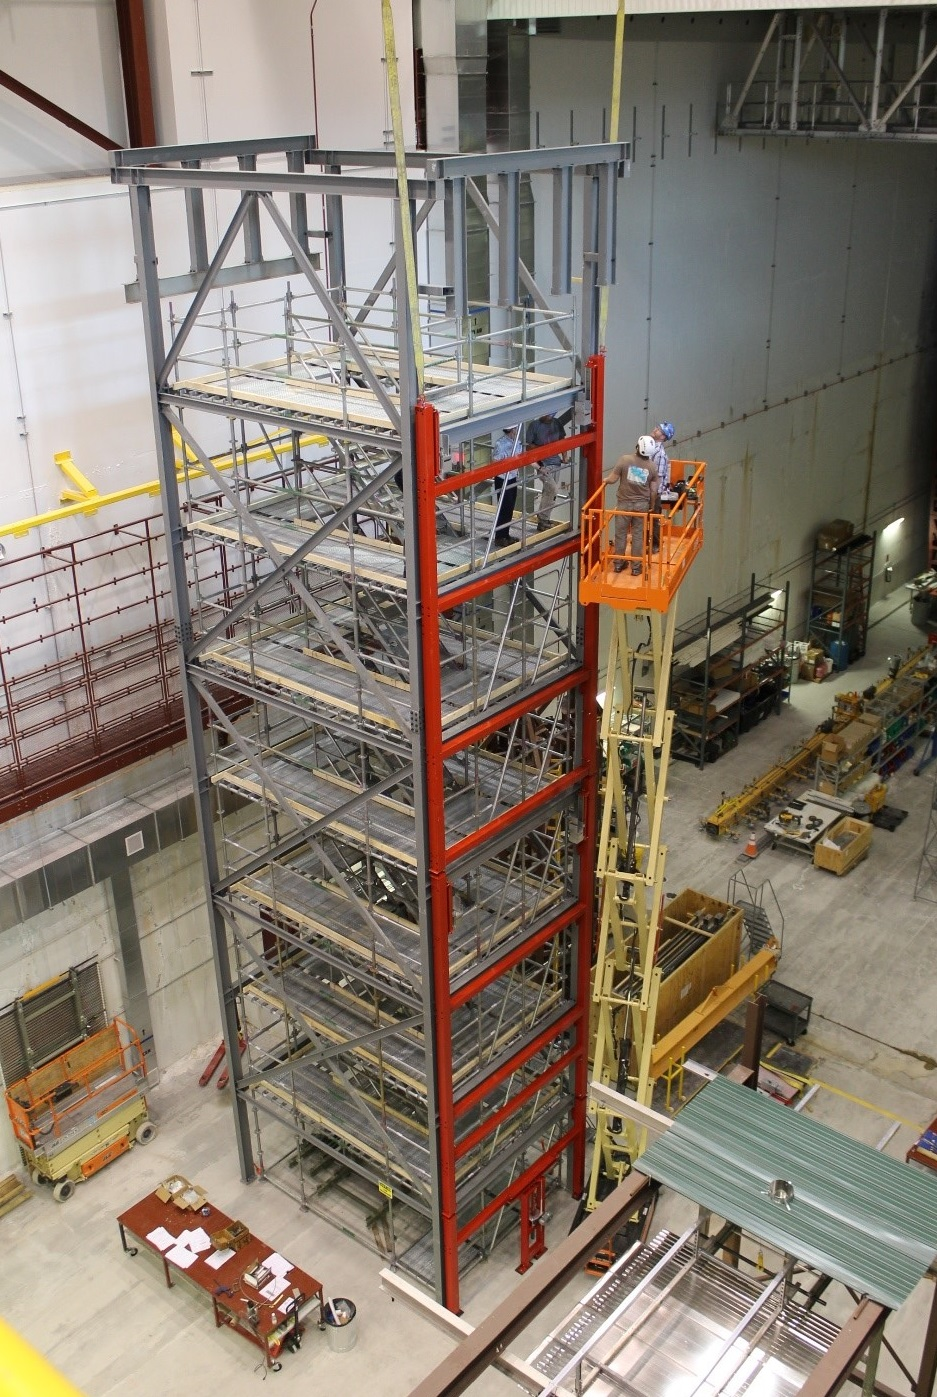
\includegraphics[width=0.65\textwidth]{ashriver_tower}
\end{dunefigure}

The work at \dword{ashriver} is divided in three major phases.
The three phases are the following:
\begin{itemize}
  \item {Phase 0:} A vertical cabling test using two full-scale 
         \dword{apa} side tubes connected top to bottom and mounted 
         against a vertical column in the detector hall.  Using this 
         setup the proposed cable bundles have been run through the 
         tubes to see how well the designed conduit system functions.
         This work has led to several proposed modifications to the 
         designs which are currently being considered.  The older 
         \dword{protodune} trial assembly structure is concurrently 
         being used to perform mechanical tests of \dword{protodune2} 
         components. 
  \item {Phase 1:} A prototype of the \dword{dune} \dword{apa} 
         assembly tower using a steel frame large enough to hold a 
         commercial stair scaffold within its mid-section as shown 
         in Figure~\ref{fig:ashriver1} is being constructed.  The 
         tower is designed to test the process for connecting top 
         and bottom \dword{apa} pairs together and installing the 
         required cable bundles.  The next step will be to add a
         \dword{cpa} assembly station and test assembly procedures 
         for the updated \dword{cpa} designs.  A prototype 
         \dword{apa} shipping frame is also being constructed to 
         test the mechanical features of the shipping container 
         design.  
  \item {Phase 2:} A more complex steel structure will be 
         designed and fabricated to mock up the network of rails 
         and support structures used to install the \dword{dune}
         \dword{fd} modules including pieces of the \dword{dss}, 
         which sits inside the cryostat.  This structure as 
         illustrated in Figure~\ref{fig:ashriver2} will provide 
         a platform for performing more detailed tests of the 
         proposed detector installation plan.  Installation steps 
         to be tested include \dword{dss} installation, transfer 
         of \dword{tpc} components through the \dword{tco}, 
         installation of the \dword{tpc} end walls, cabling 
         through the cryostat penetrations, movement of the 
         \dword{apa} and  \dword{cpa} pairs into their final 
         positions, and deployment of the top and bottom field 
         cage modules.
\end{itemize}
\begin{dunefigure}[Phase 2 trial assembly at \dword{ashriver}]{fig:ashriver2}
  {Phase 2 trial assembly at \dword{ashriver}.}
  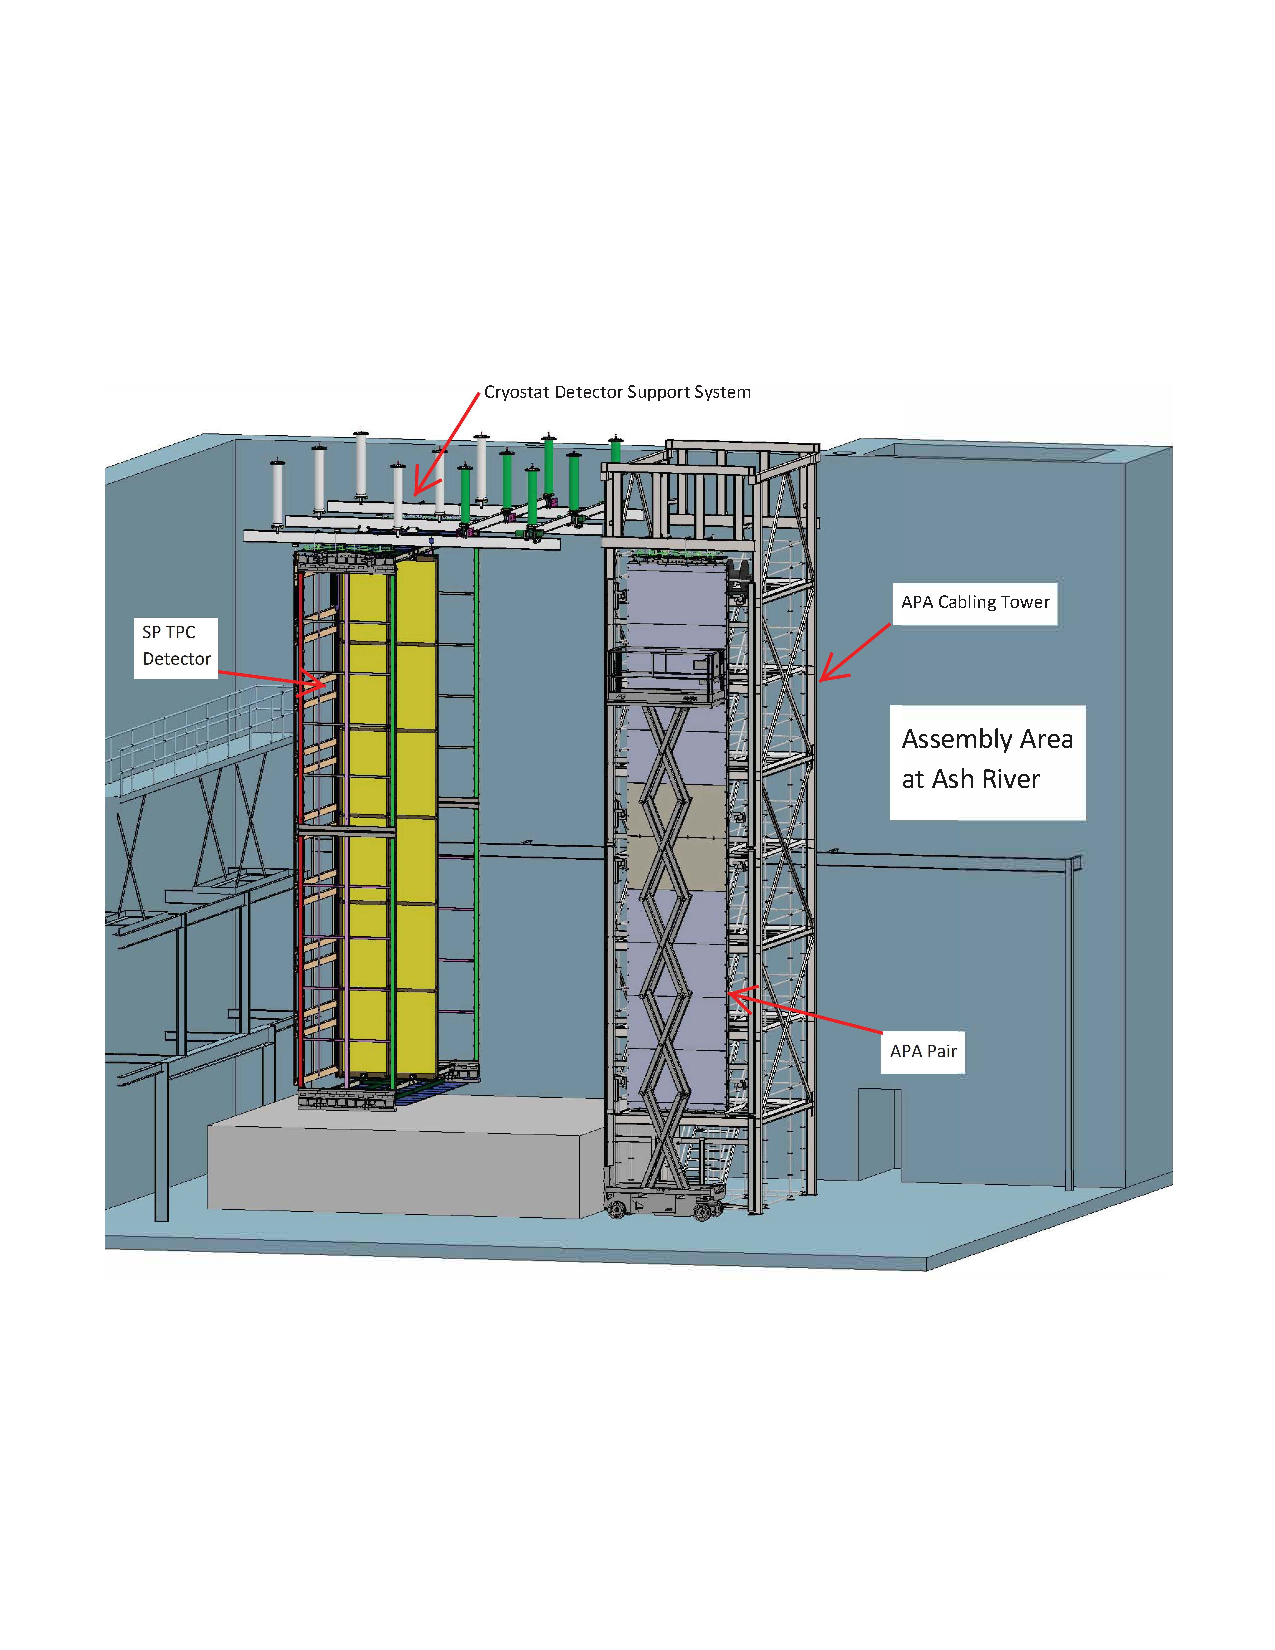
\includegraphics[width=0.65\textwidth]{Phase2_Trial_Assembly.pdf}
\end{dunefigure}

\section{South Dakota Services Division}
\label{sec:fdsp-coord-host_facility_services}

\dword{fnal} has established the \dword{sdsd} to support integration
and installation activities in South Dakota. \dword{sdsd} will support
these activities, which are the responsibility of the \dword{ipd}, by
providing access to the required technical resources.  These resources
include dedicated \dword{fnal} personnel sitting within the division
and contracted labor provided through the division.  In analogy with
the Ash River site, where University of Minesota officials are
responsible for any building permits, \dword{sdsd} is responsible for
any electrical or building permits in the leased space at \dword{surf}.

\dword{sdsd} is responsible for badging and access to the leased areas
at \dword{surf} in coordination with the \fnal Global Services Office
and the \dword{surf} Administrative Services Office. This includes
providing and coordinating the trainings required to access surface
and underground areas.  \dword{sdsd} also takes on the responsibility
for performing regular inspections and maintenance of
\dword{lbnf-dune} equipment at \dword{surf} including lifts,
conveyances, networking equipment, cooling and ventillation equipment,
electrical power installations, life safety systems, and controlled
access equipment.  Contracts that need to be written for conventional
facilities procurements after the \dword{lbnf} conventional facilities
contractor leaves the site will also be handled through the
\dword{sdsd}.
